\documentclass[12pt,a4paper,frenchb]{article}

\input{../../commons.tex.inc}

\makeatletter

\renewcommand{\maketitle}%
{\framebox{%
    \begin{minipage}{1.0\linewidth}%
      \begin{center}%
        \Large \@title ~-- \@author \\%
        \@date%
      \end{center}%
    \end{minipage}}%
  \normalsize%
  %\vspace{1cm}%
}

\makeatother

\setlength{\parsep}{0pt}
\setlength{\parskip}{5pt}
\setlength{\parindent}{0pt}
\setlength{\itemsep}{7pt}

\everymath{\displaystyle\everymath{}}

\title{Probabilités sur un ensemble fini}
\author{Terminale S}
\date{septembre 2017}

\begin{document}

\maketitle

\section{Conditionnement}
\subsection{Probabilités conditionnelles}

Soit $A$ et $B$ deux parties non vides d'un espace de probabilité
$\Omega$. On admet, qu'alors, $p(A)$ et $p(B)$ sont tous deux différents
de 0.

\begin{definition}
  On appelle \emph{probabilité conditionnelle de $B$ sachant $A$} le
  nombre, noté $p_A(B)$, $\dfrac{p(A\cap B)}{p(A)}$.
\end{definition}

\begin{remarque}
  On note aussi $p(A|B)$.
\end{remarque}

\begin{propriete}
  On a aussi $p(A\cap B) = p_A(B) \times p(A)$.
\end{propriete}

\subsection{L'arbre pondéré de probabilité}

L'arbre de probabilité correctement construit constitue une preuve !

En voici un exemple :

\begin{center}
  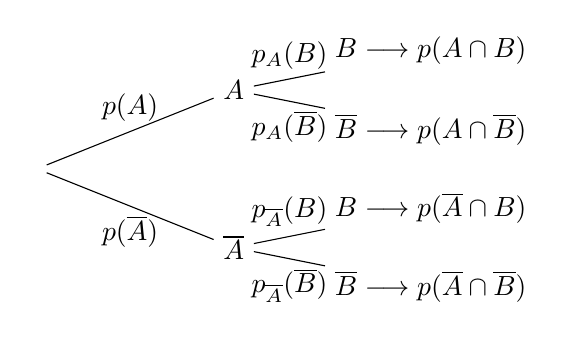
\begin{tikzpicture}[level distance=25mm,sibling distance=10mm]
    \node {} [grow=right]
    child[sibling distance=20mm] {
      node {$\overline{A}$}
      child[sibling distance=10mm] {
        node {$\overline{B} \longrightarrow p(\overline{A}\cap\overline{B})$}
        edge from parent node[below] {$p_{\overline{A}}(\overline{B})$}
      }
      child[sibling distance=10mm] {
        node {$B \longrightarrow p(\overline{A} \cap B)$}
        edge from parent node[above] {$p_{\overline{A}}(B)$}
      }
      edge from parent node[below] { $p(\overline{A})$ }
    }
    child[sibling distance=20mm] { node {$A$}
      child[sibling distance=10mm] {
        node {$\overline{B} \longrightarrow p(A\cap\overline{B})$}
        edge from parent node[below] { $p_A(\overline{B})$ }
      }
      child[sibling distance=10mm] {
        node {$B \longrightarrow p(A\cap B)$}
        edge from parent node[above] { $p_A(B)$ }
      }
      edge from parent node[above] { $p(A)$ }
    } ;
  \end{tikzpicture}
\end{center}

Afin de retrouver la probabilité de $B$, on a besoin de la formule des
partitions. Précisons les termes employés.

\begin{definition}[Partition d'un ensemble]
  Soient $A_1,\dots,A_k$, $k$ sous ensembles d'un ensemble $\Omega$.

  On dit que $(A_i)_{1\leq i\leq k}$ forment une \emph{partition} de
  $\Omega$ si et seulement si
  \begin{itemize}
    \item $\bigcup_{i=1}^k A_i = \Omega$
    \item $\forall (i,j) \in [1,k]\cap\N,\  i\neq j \implies A_i\cap
      A_j = \emptyset$
  \end{itemize}
\end{definition}

\begin{remarque} $A$ et son complémentaire $\overline{A}$ forment une
  partition de $\Omega$.
\end{remarque}

\begin{propriete}[«Distributivité» ensembliste]
  Soient $A$, $B$ et $C$, trois sous ensembles distincts de $\Omega$.

  \begin{itemize}
    \item $(A \cup B) \cap C = (A\cap C) \cup (B\cap C)$
    \item $(A \cap B) \cup C = (A \cup C) \cap (B \cup C)$
  \end{itemize}
\end{propriete}

\framebox{
  \begin{minipage}{0.99\linewidth}
    \emph{Preuve :}
      \vspace{6cm}
  \end{minipage}
}

\begin{remarque}~

  Soient $A$ et $B$ deux parties de $\Omega$.

  Si $B \subset A$, alors $A\cap B = B$ et $A\cup B= A$.
\end{remarque}

\begin{propriete}[formule des partitions]
  Soit $(A_i)_{1\leq i\leq k}$ une partition de $\Omega$

  $p(B) = \sum_{i=1}^k p(A_i \cap B)$
\end{propriete}

\framebox{
  \begin{minipage}{0.99\linewidth}
    \emph{Écrire $P(B)$ en fonction des probabilités conditionnés par
    les $A_i$ de la partition :}
    \vspace{3cm}
  \end{minipage}
}

\framebox{
  \begin{minipage}{0.99\linewidth}
    \emph{Appliquer l'écriture précédente à la partition triviale
    $(A;\overline{A})$ :}
    \vspace{3cm}
  \end{minipage}
}

\pagebreak

\section{Indépendance}

\begin{propriete}
  Soient deux événements $A$ et $B$ de probabilités non nulles.
  $p_B(A) = p(A) \iff p_A(B) = p(B)$
\end{propriete}

\framebox{
  \begin{minipage}{0.99\linewidth}
    \emph{Preuve :}
      \vspace{4cm}
  \end{minipage}
}

On dit que deux événéments sont indépendants, lorsque l'un ne
conditionne pas l'autre, c'est à dire que $p_A(B) = p(B)$.

On a donc le théorème suivant :

\begin{theoreme}[Indépendance]
  Soient $A$ et $B$ deux événements. $A$ et $B$ sont indépendants si et
  seulement si $p(A\cap B) = p(A)\times p(B)$
\end{theoreme}

\begin{propriete}
  Soient $A$ et $B$ deux événements indépendants.

  Dans ce cas, $\overline{A}$ et $B$ sont aussi indépendants.
\end{propriete}

\framebox{
  \begin{minipage}{0.99\linewidth}
    \emph{Preuve :}
      \vspace{4cm}
  \end{minipage}
}


\end{document}
